\documentclass{beamer}
\usepackage[latin1]{inputenc}
\usepackage[spanish]{babel}
\usepackage{amsmath,amsfonts}
\usepackage{bm}
\newcommand{\diver}{\operatorname{{\bf div}}}
\mode<presentation>
{
  \usetheme{PaloAlto}
  % or ...

%  \setbeamercovered{transparent}
  % or whatever (possibly just delete it)
  \usecolortheme{default}
}

\title[Elasticidad lineal]{
MÉTODO DE LOS ELEMENTOS FINITOS. \\
Elasticidad lineal}
\author[F. Gabaldón]{Felipe Gabaldón Castillo}
\date{}
\pgfdeclareimage[height=0.5cm]{logo-upm}{upm}
\logo{\pgfuseimage{logo-upm}}

\AtBeginSection[]
{
  \begin{frame}<beamer>
    \frametitle{Índice}
    \tableofcontents[currentsection]
  \end{frame}
}
%%%%%%%%%%%%%%%%%%%%%%%%%%%%%%%%%%%%%%%%%%%%%%%%%%%%%%%%%%%%%%%%%%%%%%%%%%%%%%
\newcommand{\norm}[1]{\lVert #1 \rVert}
\begin{document}
%%%%%%%%%%%%%%%%%%%%%%%%%%%%%%%%%%%%%%%%%%%%%%%%%%%%%%%%%%%%%%%%%%%%%%%%%%%%%%
\begin{frame}
\titlepage
\end{frame}
%%%%%%%%%%%%%%%%%%%%%%%%%%%%%%%%%%%%%%%%%%%%%%%%%%%%%%%%%%%%%%%%%%%%%%%%%%%%%%
\begin{frame}
\frametitle{Índice}
\tableofcontents
\end{frame}
%%%%%%%%%%%%%%%%%%%%%%%%%%%%%%%%%%%%%%%%%%%%%%%%%%%%%%%%%%%%%%%%%%%%%%%%%%%%%%
\section{Introducción}
%%%%%%%%%%%%%%%%%%%%%%%%%%%%%%%%%%%%%%%%%%%%%%%%%%%%%%%%%%%%%%%%%%%%%%%%%%%%%%
\begin{frame}
\frametitle{Introducción}
\begin{itemize}
\item Sea $\bm{\sigma}$ el tensor de tensiones
de Cauchy, $\bm{u}$ el vector desplazamiento y $\bm{b}$ el vector de
fuerzas volumétricas.
\item Consideraremos el tensor de deformaciones infinitesimales, que se define
como la parte simétrica del tensor gradiente de desplazamientos:
\begin{equation}
\bm{\varepsilon}=\bm{\nabla}^s \bm{u}, \quad
\varepsilon_{ij}=u_{(i,j)}=\frac{1}{2}\left(
\frac{\partial u_i}{\partial x_j}+
\frac{\partial u_j}{\partial x_i}
\right)
\end{equation}
\item Las componentes del tensor de
tensiones se expresan como combinación lineal de las componentes del tensor
de deformaciones mediante un tensor de cuarto orden
$\boldsymbol{\mathsf{C}}$ (Ley de Hooke generalizada), cuyas
componentes $\mathsf{C}_{ijkl}$
son constantes y se denominan ``coeficientes elásticos'':
\begin{equation}
\bm{\sigma}= \boldsymbol{\mathsf{C}} \bm{\varepsilon} , \quad
\sigma_{ij}=\mathsf{C}_{ijkl} \varepsilon_{kl} \label{hookegen}
\end{equation}
\end{itemize}
\end{frame}
%%%%%%%%%%%%%%%%%%%%%%%%%%%%%%%%%%%%%%%%%%%%%%%%%%%%%%%%%%%%%%%%%%%%%%%%%%%%%%
\begin{frame}
\frametitle{Introducción}
El tensor de módulos elásticos tiene las siguientes propiedades:
\begin{enumerate}
\item Simetría mayor:
\begin{equation}
\mathsf{C}_{ijkl}=\mathsf{C}_{klij} \label{scmayor}
\end{equation}
\item Simetría menor:
\begin{align}
\mathsf{C}_{ijkl}&=\mathsf{C}_{jikl} &
\mathsf{C}_{ijkl}&=\mathsf{C}_{ijlk}
\end{align}
\item Es definido positivo:
\begin{align}
\mathsf{C}_{ijkl} \Phi_{ij} \Phi_{kl}& \geq 0 \quad \forall \Phi_{ij}
\textrm{ simétrico} \label{sfcdpos1}\\
\mathsf{C}_{ijkl} \Phi_{ij} \Phi_{kl} &=0 \quad \Rightarrow \quad
\Phi_{ij}=0 \label{sfcdpos2}
\end{align}
\end{enumerate}
Consideraremos un sólido elástico definido por un conjunto abierto
$\Omega \subset \mathbb{R}^{n_{\rm dim}}$ con contorno
$\partial \Omega$, tal que:
\begin{align}
\partial \Omega &=\partial_{u_i} \Omega \cup \partial_{t_i} \Omega &
\emptyset       &=\partial_{u_i} \Omega \cap \partial_{t_i} \Omega
\end{align}
siendo $\partial_{u_i} \Omega$ la parte del contorno con desplazamientos
impuestos en dirección $i$, y $\partial_{t_i} \Omega$ la parte con tensiones
impuestas en dirección $i$
\end{frame}
%%%%%%%%%%%%%%%%%%%%%%%%%%%%%%%%%%%%%%%%%%%%%%%%%%%%%%%%%%%%%%%%%%%%%%%%%%%%%%
\section{Formulación del problema de contorno}
%%%%%%%%%%%%%%%%%%%%%%%%%%%%%%%%%%%%%%%%%%%%%%%%%%%%%%%%%%%%%%%%%%%%%%%%%%%%%%
\begin{frame}
\frametitle{Formulación fuerte}
\parbox{70mm}{
Sea $\overline{\Omega}=\Omega \cup \partial \Omega$ el dominio
ocupado por un sólido, cuyo contorno es $\partial \Omega=
\partial_u \Omega \cup \partial_t \Omega$ con
$\partial_u \Omega \cap \partial_t \Omega=\emptyset$. La
formulación fuerte del problema se establece en los siguientes términos:
}\parbox{60mm}{
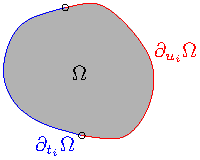
\includegraphics{elas1}
}
Dados $\bm{b}:\overline{\Omega} \rightarrow \mathbb{R}^n$,
$\overline{\bm{u}}: \partial_u \Omega \rightarrow \mathbb{R}^n$,
$\overline{\bm{t}}: \partial_t \Omega \rightarrow \mathbb{R}^n$,
encontrar el campo de desplazamientos $u\in \mathbb{R}^n$ que cumple:
\begin{align}
\diver\bm{\sigma}+\bm{b}&=0  \qquad \textrm{ en }\;{\Omega} \label{eula11} \\
\bm{\sigma}\bm{n}&=\overline{\bm{t}} \qquad \textrm{ en }\;\partial_t \Omega \\
\bm{u}&=\overline{\bm{u}} \qquad \textrm{ en }\;\partial_u \Omega
\end{align}
con $\bm{\sigma}=\frac{\partial W}{\partial \bm \varepsilon}$ y
$\bm{\varepsilon}=\bm{\nabla}^{S}\bm{u}$
\end{frame}
%%%%%%%%%%%%%%%%%%%%%%%%%%%%%%%%%%%%%%%%%%%%%%%%%%%%%%%%%%%%%%%%%%%%%%%%%%%%%%
\begin{frame}
\frametitle{Formulación débil}
Dados $\bm{b}:\overline{\Omega}\rightarrow \mathbb{R}^n$ y las funciones
$\overline{\bm{u}}:\partial_u \Omega \rightarrow \mathbb{R}^n$,
$\overline{\bm{t}}:\partial_t \Omega \rightarrow \mathbb{R}^n$,
encontrar el campo de
desplazamientos $\bm{u}\in \delta\,\mid \, \forall \delta \bm{u} \in {\cal V}$
cumple:
\begin{equation}
\int_{\Omega}\left( \bm{\sigma}\cdot \bm{\nabla}^{S}\delta \bm{u}
-\bm{b} \cdot \delta \bm{u} \right) \, d \Omega
-\int_{\partial_t \Omega} \overline{\bm{t}}\cdot
\delta \bm{u} \, d \Gamma =0 \label{formdeb}
\end{equation}
siendo:
\begin{align}
\delta&=\left\{
\bm{u} \in H^1(\Omega,\mathbb{R}^n) \mid \bm{u}(\bm{x})=\overline{\bm{u}}
\; \quad \forall \; \bm{x} \in \partial_u \Omega \right\} \label{trial} \\
{\cal V}&=\left\{
\delta \bm{u} \in H^1(\Omega,\mathbb{R}^n) \mid \delta \bm{u}(\bm{x})=\bm
{0} \; \quad \forall \; \bm{x} \in \partial_u \Omega \right\} \label{weight}
\end{align}
y $H^1(\Omega,\mathbb{R}^n)$ el espacio de Sobolev de orden $1$ y grado $2$:
$$
H^1=\left\{ \bm{u}:\Omega \rightarrow \mathbb{R}^n \quad \mid \quad
\int_{\Omega} \norm{\bm{u}}_{2,1} \, d\Omega <\infty \right\}
$$
\end{frame}
%%%%%%%%%%%%%%%%%%%%%%%%%%%%%%%%%%%%%%%%%%%%%%%%%%%%%%%%%%%%%%%%%%%%%%%%%%%%%%
\begin{frame}
\frametitle{Equivalencia de ambas formulaciones}
\begin{itemize}
\item Lema 1. Descomposición euclídea de un tensor de orden 2
\begin{equation*}
s_{ij}=\underbrace{s_{(ij)}}_{\textrm{simétrico}}+
       \underbrace{s_{[ij]}}_{\textrm{hemisimétrico}};
\quad
s_{(ij)}=\frac{s_{ij}+s_{ji}}{2},
\;
s_{[ij]}=\frac{s_{ij}-s_{ji}}{2}
\end{equation*}
\item Lema 2. Sea $s_{ij}$ un tensor simétrico y $t_{ij}$ un tensor no 
simétrico. Entonces,
$$
s_{ij} t_{ij}=s_{ij} t_{(ij)}
$$
El lema queda demostrado si $s_{ij} t_{[ij]}=0$. En efecto:
\begin{align*}
s_{ij} t_{[ij]}&=-s_{ij} t_{[ji]} \\
\mbox{}        &=-s_{ji} t_{[ji]} \\
\mbox{}        &=-s_{ij} t_{[ij]}
\end{align*}
\end{itemize}
\end{frame}
%%%%%%%%%%%%%%%%%%%%%%%%%%%%%%%%%%%%%%%%%%%%%%%%%%%%%%%%%%%%%%%%%%%%%%%%%%%%%%
\begin{frame}
\frametitle{Equivalencia de ambas formulaciones}
Si $\bm{u}$ es solución del problema fuerte, 
multiplicando (\ref{eula11}) por $\delta \bm{u} \in {\cal V}$ e integrando en
$\Omega$:
\begin{align}
0&= \int_{\Omega} (\sigma_{ij,j}+b_i)\delta u_i d\Omega \nonumber \\
 &= \int_{\Omega} (\sigma_{ij}\delta u_i)_{,j} d \Omega -
    \int_{\Omega}  \sigma_{ij}\delta u_{i,j} d \Omega +  
    \int_{\Omega} b_i \delta u_i d\Omega \nonumber \\
 &=-\int_{\Omega} \sigma_{ij}\delta u_{(i,j)} d \Omega +
    \int_{\Omega}  b_i \delta u_i d\Omega + 
    \int_{\partial_{t_i}\Omega}  \overline{t}_i \delta u_i d \Gamma
\end{align}
y por tanto $u_i$ es solución del problema débil
\end{frame}
%%%%%%%%%%%%%%%%%%%%%%%%%%%%%%%%%%%%%%%%%%%%%%%%%%%%%%%%%%%%%%%%%%%%%%%%%%%%%%
\begin{frame}
\frametitle{Equivalencia de ambas formulaciones}
Sea $u_i$ solución del problema débil. Dado que $u_i \in \delta_i$, $u_i=
\overline{u}_i$ en $\partial_{u_i} \Omega$. De (\ref{formdeb}):
\begin{align}
0&=-\int_{\Omega} \sigma_{ij}\delta u_{i,j} d \Omega +
  \int_{\Omega}  b_i \delta u_i d\Omega +
  \int_{\partial_{t_i}\Omega}  \overline{t}_i \delta u_i d \Gamma \nonumber \\
 &=-\int_{\Omega} (\sigma_{ij}\delta u_i)_{,j} d \Omega +
  \int_{\Omega} (\sigma_{ij,j}+b_i)\delta u_i d \Omega +
  \int_{\partial_{t_i}\Omega}  \overline{t}_i \delta u_i d \Gamma \nonumber \\
 &= \int_{\Omega} (\sigma_{ij,j}+b_i)\delta u_i d \Omega -
  \int_{\partial_{t_i}\Omega}(\sigma_{ij}n_j-\overline{t}_i)\delta u_i d \Gamma
\label{demoeq}
\end{align}
\end{frame}
%%%%%%%%%%%%%%%%%%%%%%%%%%%%%%%%%%%%%%%%%%%%%%%%%%%%%%%%%%%%%%%%%%%%%%%%%%%%%%
\begin{frame}
\frametitle{Equivalencia de ambas formulaciones}
Sean:
\begin{align}
\alpha_i&=\sigma_{ij,j}+b_i \\
\beta_i&=\sigma_{ij}n_j-\overline{t}_i
\end{align}
La equivalencia entre ambas formulaciones estará demostrada si se verifica
que $\alpha_i=0$ en $\Omega$ y $\beta_i=0$ en $\partial_{t_i} \Omega$.
Sea $\delta u_i=\alpha_i \phi$, donde:
\begin{align*}
\phi&>0 \textrm{ en } \Omega \\
\phi&=0 \textrm{ en } \partial \Omega \\
\phi& \textrm{ suave}
\end{align*}
Con estas condiciones queda garantizado que $\delta u_i \in {\cal V}$.
\end{frame}
%%%%%%%%%%%%%%%%%%%%%%%%%%%%%%%%%%%%%%%%%%%%%%%%%%%%%%%%%%%%%%%%%%%%%%%%%%%%%%
\begin{frame}
\frametitle{Equivalencia de ambas formulaciones}
Sustituyendo este $\delta u_i$ en (\ref{demoeq}):
\begin{equation}
0=\int_{\Omega} \underbrace{\alpha_i \, (\alpha_i}_{\geq 0}
\underbrace{ \phi}_{>0}) d\Omega 
\Rightarrow \quad \alpha_i=0 \textrm{ en } \Omega
\end{equation}
Análogamente, tomemos ahora $\delta u_i=\delta_{i1} \beta_1 \psi$, donde:
\begin{align*}
\psi&>0 \textrm{ en } \partial_{t_1}\Omega \\
\psi&=0 \textrm{ en } \partial_{u_1} \Omega \\
\psi& \textrm{ suave}
\end{align*}
Sustituyendo esta nueva expresión de $\delta u_i \in {\cal V}$ en
(\ref{demoeq}):
\begin{equation}
0=\int_{\partial_{t_1} \Omega} \underbrace{\beta_1 \, (\beta_1}_{\geq 0}
\underbrace{ \psi}_{>0}) d\Omega 
\Rightarrow \quad \beta_1=0 \textrm{ en } \partial_{t_1} \Omega
\end{equation}
\end{frame}
%%%%%%%%%%%%%%%%%%%%%%%%%%%%%%%%%%%%%%%%%%%%%%%%%%%%%%%%%%%%%%%%%%%%%%%%%%%%%%
\section{Formulaciones variacionales}
\begin{frame}
\frametitle{Formulaciones variacionales}
Considerando el funcional de la energía potencial:
\begin{equation}
\Pi_p(\bm{u})=
\int_{\Omega} \left(
W(\bm{x},\bm{\varepsilon})-\bm{b} \cdot \bm{u}\right) \, d \Omega
-\int_{\partial_t \Omega} \overline{\bm{t}}\cdot\bm{u} \, d \Gamma\label{potenc}
\end{equation}
la ecuación (\ref{formdeb}) equivale a establecer la condición de
estacionariedad del funcional (\ref{potenc}):
\begin{equation}
\delta \Pi_p(\bm{u})=0 \label{potest}
\end{equation}
\begin{itemize}
\item Se dice que (\ref{formdeb}) es la ecuación variacional del problema
(\ref{potest}), y que las ecuación (\ref{eula11}) es la ecuación de
Euler-Lagrange asociada al problema variacional (\ref{potest}).
\item Para la ley de Hooke:
\begin{equation}
W(\bm{x},\bm{\varepsilon})=\frac{1}{2} \bm{\varepsilon} \cdot 
\bm{\mathsf{C}} \bm{\varepsilon}
\end{equation}
\end{itemize}
\end{frame}
%%%%%%%%%%%%%%%%%%%%%%%%%%%%%%%%%%%%%%%%%%%%%%%%%%%%%%%%%%%%%%%%%%%%%%%%%%%%%%
\begin{frame}
\frametitle{Formulaciones variacionales}
\begin{itemize}
\item Existen otros principios variacionales diferentes al expresado en
(\ref{potest}), asociado al funcional de la {\em energía potencial
total} (\ref{potenc}).
\item Dichos principios son la base de la formulación de
los denominados ``elementos mixtos''.
\item En general se deducen a partir de ``funcionales multicampo'' como,
por ejemplo, el de Hu-Washizu:
\begin{multline*}
\Pi_W(\bm{u},\bm{\varepsilon},\bm{\sigma})=
\int_{\Omega} \left(
W(\bm{x},\bm{\varepsilon})-\bm{\sigma}\cdot\bm{\varepsilon}+
\bm{\sigma}\cdot\bm{\nabla}^{S}\bm{u}-\bm{b} \cdot \bm{u}\right) \, d \Omega \\
-\int_{\partial_t \Omega} \overline{\bm{t}}\cdot\bm{u} \, d \Gamma\label{hu-was}
\end{multline*}
\end{itemize}
\end{frame}
%%%%%%%%%%%%%%%%%%%%%%%%%%%%%%%%%%%%%%%%%%%%%%%%%%%%%%%%%%%%%%%%%%%%%%%%%%%%%%
\section{Formulación de Galerkin}
\begin{frame}
\frametitle{Formulación de Galerkin}
\begin{itemize}
\item Sean $\nu^h$ y $\delta^h$ aproximaciones de dimensión finita de los
espacios funcionales $\nu$ y $\delta$, respectivamente
\item Se adopta la descomposición: $\bm{u}^h=\bm{v}^h+\overline{\bm{u}}^h$
con $\bm{v}^h \in \nu^h$ y 
$\overline{\bm{u}}^h=\overline{\bm{u}}$ en $\partial_u \Omega$ (``aproximadamente'')
\item Dados $\bm{b}:\overline{\Omega}\rightarrow \mathbb{R}^n$ y las funciones
$\overline{\bm{u}}:\partial_u \Omega  \rightarrow \mathbb{R}^n$,\, 
$\overline{\bm{t}}:\partial_t \Omega  \rightarrow \mathbb{R}^n$, 
encontrar el campo de
desplazamientos $\bm{u}^h=\bm{v}^h+\overline{\bm{u}}^h$, con $\delta \bm{v}^h
\in \nu^h$, tal que
$\forall \delta \bm{u}^h \in \nu^h$ se cumple:
\begin{equation}
\begin{split}
\int_{\Omega}
\bm{\nabla}^{S} \bm{v}^h \cdot \bm{\mathsf{C}}
\bm{\nabla}^{S}\delta \bm{u}^h \, d \Omega
=\int_{\Omega} \bm{b} \cdot \delta \bm{u}^h \, d \Omega
+\int_{\partial_t \Omega} \overline{\bm{t}}\cdot
\delta \bm{u}^h \, d \Gamma \\
-\int_{\Omega} \bm{\nabla}^{S} \overline{\bm{u}}^h \cdot \bm{\mathsf{C}}
\bm{\nabla}^{S}\delta \bm{u}^h \, d \Omega
\end{split}
\label{ecvapr1}
\end{equation}
\end{itemize}
\end{frame}
%%%%%%%%%%%%%%%%%%%%%%%%%%%%%%%%%%%%%%%%%%%%%%%%%%%%%%%%%%%%%%%%%%%%%%%%%%%%%%
\section{Formulación de Elementos Finitos}
\begin{frame}
\frametitle{Formulación de elementos finitos}
\begin{itemize}
\item El dominio $\Omega$ se discretiza en $n_{\textrm{elm}}$ elementos
$\Omega^e$:
\begin{equation}
\Omega=\bigcup_{e=1}^{n_{\textrm{elm}}} \Omega^e \qquad \Omega^i \cap \Omega^j=
\emptyset,\textrm{ si } i\neq j
\end{equation}
\item El elemento $\Omega^e$ se transforma
en un ``cubo unitario''
$$\Box=\underbrace{[-1,1]\times \cdots \times [-1,1]}_{n_{\rm dim}}$$
definido en el espacio isoparamétrico de coordenadas $\{ \bm{\xi} \}$:
\begin{equation}
\bm{\phi}:\bm{\xi}\in \Box \rightarrow \bm{x} \in \Omega^e; \qquad
\bm{x}=\bm{\phi}(\bm{\xi})=\sum_{A=1}^{n^{e}_{\textrm{nod}}}
\bm{x}_{A} N_{A}(\bm{\xi}) \label{mapiso}
\end{equation}
siendo $\bm{x}_A$ las coordenadas de los nodos
del elemento $e$
\end{itemize}
\end{frame}
%%%%%%%%%%%%%%%%%%%%%%%%%%%%%%%%%%%%%%%%%%%%%%%%%%%%%%%%%%%%%%%%%%%%%%%%%%%%%%
\begin{frame}
\frametitle{Formulación de elementos finitos}
\begin{itemize}
\item Los subespacios de dimensión finita $\delta^h$ y ${\cal V}^h$
se definen mediante unas funciones de interpolación $N_A, \;
A=1 \ldots n_{\textrm{nod}}$ (polinómicas), que se denominan ``funciones de forma''
\begin{small}
\begin{align*}
\delta^h&=\left\{
\bm{u}^{h} \in \delta \mid
u_i^{h}=\sum_{A\in \eta - \eta_{u_i}} u_{iA}N_{A}(\bm{\xi})+
\sum_{A \in \eta_{u_i}} \overline{u}_{iA}N_{A}(\bm{\xi})
\right\}  \\
{\cal V}^{h}&=\left\{
\delta \bm{u}^{h} \in {\cal V} \mid \delta u_i^{h}=0 \;\;
\forall \bm{x} \in \partial_{u_i} \Omega ; \quad
\delta u_i^{h}=\sum_{A\in \eta - \eta_{u_i}}
\delta u_{iA}N_{A}(\bm{\xi})
\right\}
\end{align*}
\end{small}
siendo $\eta=\{ 1,2,\ldots,n_{\textrm{numnp}} \}$ el conjunto de números de los
$n_{\textrm{numnp}}$ nodos de la malla, $\eta_{u_i} \subset \eta$ el conjunto
de nodos en los que $u_i^h=\overline{u}_i$, y $\eta - \eta_{u_i}$ el conjunto
complementario de $\eta_{u_i}$
\end{itemize}
\end{frame}
%%%%%%%%%%%%%%%%%%%%%%%%%%%%%%%%%%%%%%%%%%%%%%%%%%%%%%%%%%%%%%%%%%%%%%%%%%%%%%
\section{Formulación matricial}
\begin{frame}
\frametitle{Interpolación del campo de desplazamientos}

Si se emplea una formulación isoparamétrica que interpola los
desplazamientos con la misma interpolación que las coordenadas
(\ref{mapiso}):
\begin{equation}
\bm{u}^h=\sum_{A=1}^{n^e_{\textrm{nod}}}
\bm{d}_{A} N_{A}(\bm{\xi}) = \mathbf{N}^{T} \bm{d}^e \label{disiso}
\end{equation}
siendo $\bm{d}^e$ el vector de desplazamientos nodales del elemento $e$
y $\mathbf{N}$ la matriz de funciones de forma del elemento. Por ejemplo, en
$2$D:
\begin{small}
\begin{equation}
\left\{
\begin{array}{c}
u_1(x,y) \\
u_2(x,y) 
\end{array}
\right\}=
\left(
\begin{array}{ccccccc}
N_1 &  0  & N_2 &  0  & \ldots & N_{\textrm n_{nod}} & 0                    \\
0   & N_1 &  0  & N_2 & \ldots &           0          & N_{\textrm n_{nod}}
\end{array}
\right) \bm{d}^e
\label{indisge}
\end{equation}
\end{small}
\end{frame}
%%%%%%%%%%%%%%%%%%%%%%%%%%%%%%%%%%%%%%%%%%%%%%%%%%%%%%%%%%%%%%%%%%%%%%%%%%%%%%
\begin{frame}
\frametitle{Interpolación del campo de deformaciones}

Con la notación en que las tensiones y
deformaciones se expresan en forma de vector (por ejemplo en 2D:
$\bm{\varepsilon}=(\varepsilon_{xx},\varepsilon_{yy},2
\varepsilon_{xy})^T$) y derivando (\ref{disiso}), la interpolación del campo
de deformaciones se expresa:
\begin{small}
\begin{equation}
\nabla^S u^h_{ij}=\sum_{A=1}^{n^e_{\textrm{nod}}}
\frac{1}{2}\left(N^e_{A,i} d_{Aj}+N^e_{A,j} d_{Ai}
\right) \Rightarrow
\bm{\nabla}^{S}\bm{u}^h=\mathbf{B} \bm{d}^e \label{intdefcomp}
\end{equation}
\end{small}
En $2$D:
\begin{small}
\begin{equation}
\bm{\varepsilon}=
\left(
\begin{array}{ccccccc}
\frac{\partial N_1}{\partial x_1} & 0 &\frac{\partial N_2}{\partial x_1} &0 &
\ldots & \frac{\partial N_{\textrm n_{nod}}}{\partial x_1} & 0 \\
0 & \frac{\partial N_1}{\partial x_2} & 0 &\frac{\partial N_2}{\partial x_2} &
\ldots & 0 & \frac{\partial N_{\textrm n_{nod}}}{\partial x_2} \\
\frac{\partial N_1}{\partial x_2} &\frac{\partial N_1}{\partial x_1} &
\frac{\partial N_2}{\partial x_2} &\frac{\partial N_2}{\partial x_1} &
\ldots & \frac{\partial N_{\textrm n_{nod}}}{\partial x_2} &\frac{\partial
N_{\textrm n_{nod}}}{\partial x_1}
\end{array}
\right)\bm{d}^e
\end{equation}
\end{small}
\end{frame}
%%%%%%%%%%%%%%%%%%%%%%%%%%%%%%%%%%%%%%%%%%%%%%%%%%%%%%%%%%%%%%%%%%%%%%%%%%%%%%
\begin{frame}
\frametitle{Ecuaciones de elementos finitos}
Sustituyendo (\ref{disiso}) y (\ref{intdefcomp}) en (\ref{ecvapr1})
e imponiendo que los desplazamientos virtuales $\delta \bm{u}$ son arbitrarios,
después de operar se obtiene:
\begin{equation}
\bm{R}\stackrel{\textrm{def}}{=}\stackrel{n_{\textrm{elm}}}{
\underset{e=1}{\mbox{\LARGE{\bf {\sf A}}}}} \left[
\bm{f}^{e,{\rm ext}}-\int_{\Omega^e}
\mathbf{B}^{T} \bm{\sigma}^{h}(\bm{\varepsilon})
\,d\Omega \right] = \bm{0} \label{resmef1}
\end{equation}
donde ${\Large \bf{\sf A}[\cdot]}$ es el operador de ensamblaje y
$\bm{f}^{e,{\rm ext}}$
es el vector de fuerzas externas convencional que se obtiene a partir de la
expresión (\ref{ecvapr1}):
\begin{equation}
\bm{f}^{e,{\rm ext}}=\int_{\Omega^e} \mathbf{N}^{T} \bm{b} d\Omega+
\int_{\partial_t \Omega^e} \mathbf{N}^{T} \overline{\bm{t}} d \Gamma
\label{fexter}
\end{equation}
\end{frame}
%%%%%%%%%%%%%%%%%%%%%%%%%%%%%%%%%%%%%%%%%%%%%%%%%%%%%%%%%%%%%%%%%%%%%%%%%%%%%%
\begin{frame}
\frametitle{Observaciones:}
\begin{itemize}
\item La ecuación (\ref{resmef1}) está planteada en forma
residual (anulando la diferencia entre las fuerzas externas y las fuerzas
internas), que es la adecuada para problemas no lineales.
\item En lo sucesivo se considerará el caso de la elasticidad lineal, en el
que si denominamos $\mathbf{C}$ a la matriz de módulos elásticos 
(o matriz constitutiva), resulta:
\begin{equation}
\bm{\sigma}^h(\bm{\varepsilon})=
\mathbf{C} \mathbf{B}\bm{d}^e
\end{equation}
entonces la ecuación (\ref{resmef1}) se expresa:
\begin{equation}
\stackrel{n_{\textrm{elm}}}{\underset{e=1}{\mbox{\LARGE{\bf {\sf A}}}}} \left[
\left(\int_{\Omega^e} \mathbf{B}^T \mathbf{C} \mathbf{B} \, d \Omega \right)
\right]\bm{d}=
\stackrel{n_{\textrm{elm}}}{\underset{e=1}{\mbox{\LARGE{\bf {\sf A}}}}}
\bm{f}^{e,\textrm{ext}} \label{linmef1}
\end{equation}
\end{itemize}
\end{frame}
%%%%%%%%%%%%%%%%%%%%%%%%%%%%%%%%%%%%%%%%%%%%%%%%%%%%%%%%%%%%%%%%%%%%%%%%%%%%%%
\begin{frame}
\frametitle{Ecuaciones de elementos finitos}
\begin{itemize}
\item La matriz de rigidez elemental se define como:
\begin{equation}
\mathbf{K}^{e}=
\int_{\Omega^{e}} \mathbf{B}^{\rm T}  \mathbf{C}
\mathbf{B} \, d \Omega \label{arrc}
\end{equation}
\item Ensamblando los vectores de fuerzas elementales y las matrices de
rigidez elementales:
\begin{align}
\bm{f}&=\stackrel{n_{\textrm{elm}}}{\underset{e=1}{\mbox{\LARGE{\bf {\sf A}}}}}
\bm{f}^{e,\textrm{ext}} \\
\mathbf{K}&=\stackrel{n_{\textrm{elm}}}{\underset{e=1}{\mbox{\LARGE{\bf {\sf A}}}}} \mathbf{K}^{e}
\end{align}
el sistema (\ref{linmef1}) se expresa:
\begin{equation}
\mathbf{K} \bm{d}=\bm{f} \Rightarrow \qquad \bm{d}=\mathbf{K}^{-1} \bm{f}
\end{equation}
\end{itemize}
\end{frame}
%%%%%%%%%%%%%%%%%%%%%%%%%%%%%%%%%%%%%%%%%%%%%%%%%%%%%%%%%%%%%%%%%%%%%%%%%%%%%%
\section{Elasticidad lineal}
\begin{frame}
\frametitle{Ecuaciones de la elasticidad lineal}

\parbox{0.3\textwidth}{
\begin{align*}
\varepsilon_x&=\frac{\sigma_x}{E}-\nu \frac{\sigma_y}{E}-\nu \frac{\sigma_z}{E}
\\
\varepsilon_y&=\frac{\sigma_y}{E}-\nu \frac{\sigma_x}{E}-\nu \frac{\sigma_z}{E}
\\
\varepsilon_z&=\frac{\sigma_z}{E}-\nu \frac{\sigma_x}{E}-\nu \frac{\sigma_y}{E}
\\
\varepsilon_{yz}&=\frac{\tau_{yz}}{2G} \\
\varepsilon_{xz}&=\frac{\tau_{xz}}{2G} \\
\varepsilon_{xy}&=\frac{\tau_{xy}}{2G} \\
\end{align*}
}\parbox{0.6\textwidth}{
\begin{itemize}
\item Módulo de corte:
$$
G=\frac{E}{2(1+\nu)}
$$
\item Deformación volumétrica
$$
e=\varepsilon_{ii}
$$
\item Módulo de def. volumétrica
\begin{align*}
e&=\frac{1-2\nu}{E}\sigma_{ii} \Rightarrow p=-k e \\
k&=\frac{E}{3(1-2\nu)}
\end{align*}
\end{itemize}
}
\end{frame}
%%%%%%%%%%%%%%%%%%%%%%%%%%%%%%%%%%%%%%%%%%%%%%%%%%%%%%%%%%%%%%%%%%%%%%%%%%%%%%
\begin{frame}
\frametitle{Elasticidad 2D. Deformación plana}
\begin{itemize}
\item La condición de deformación plana es $(\varepsilon_{zz}=0)$
\begin{align}
\left\{
\begin{array}{c}
\sigma_{xx} \\
\sigma_{yy} \\
\sigma_{xy}
\end{array}
\right\}&=
\left(
\begin{array}{ccc}
\lambda+2\mu & \lambda     & 0 \\
\lambda     & \lambda+2\mu & 0 \\
0           & 0       & \mu
\end{array}
\right)
\left\{
\begin{array}{c}
\varepsilon_{xx} \\
\varepsilon_{yy} \\
\varepsilon_{xy}
\end{array}
\right\} \\
\sigma_{zz}&=\nu (\sigma_{xx}+\sigma_{yy})
\end{align}
siendo $\lambda$ y $\mu$ los coeficientes de Lamé:
\begin{equation}
\lambda=\frac{\nu E}{(1+\nu)(1-2\nu)}\qquad \mu=\frac{E}{2(1+\nu)}
\end{equation}
\end{itemize}
\end{frame}
%%%%%%%%%%%%%%%%%%%%%%%%%%%%%%%%%%%%%%%%%%%%%%%%%%%%%%%%%%%%%%%%%%%%%%%%%%%%%%
\begin{frame}
\frametitle{Deformación plana: aplicaciones}
\begin{center}
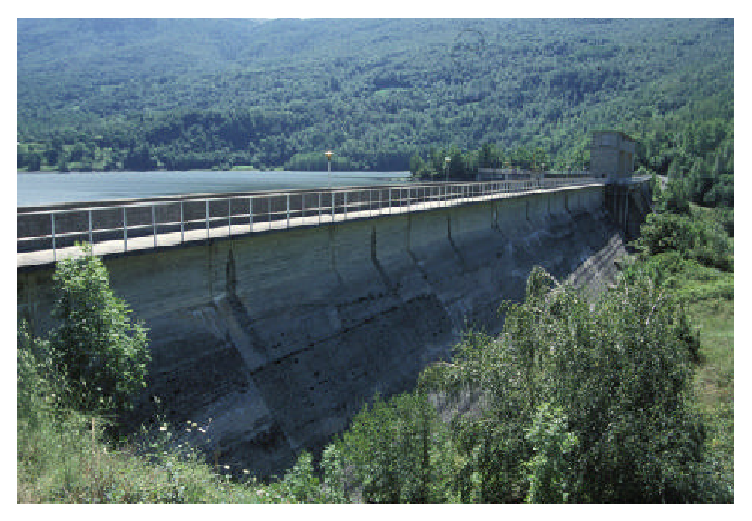
\includegraphics[width=0.85\textwidth]{damgrav}
\end{center}
\end{frame}
%%%%%%%%%%%%%%%%%%%%%%%%%%%%%%%%%%%%%%%%%%%%%%%%%%%%%%%%%%%%%%%%%%%%%%%%%%%%%%
\begin{frame}
\frametitle{Deformación plana: aplicaciones}
\begin{center}
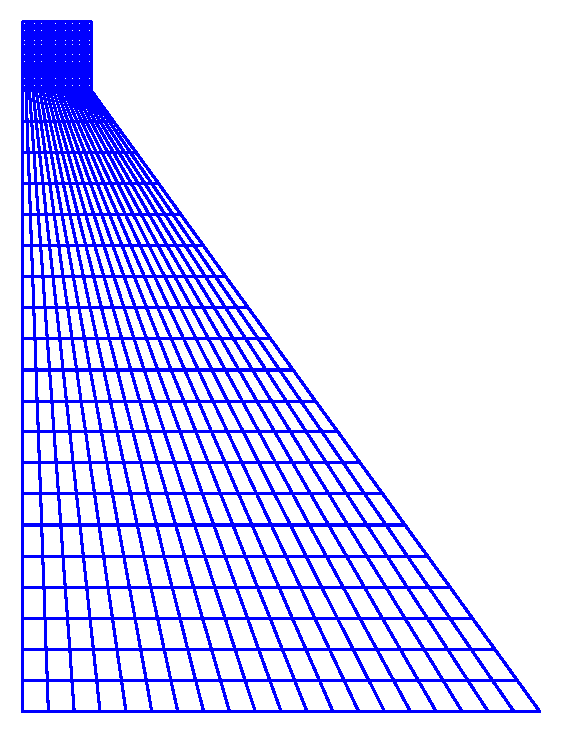
\includegraphics[width=0.40\textwidth]{dam2dm}
\hfill

\includegraphics[width=0.40\textwidth]{dam2dc1}
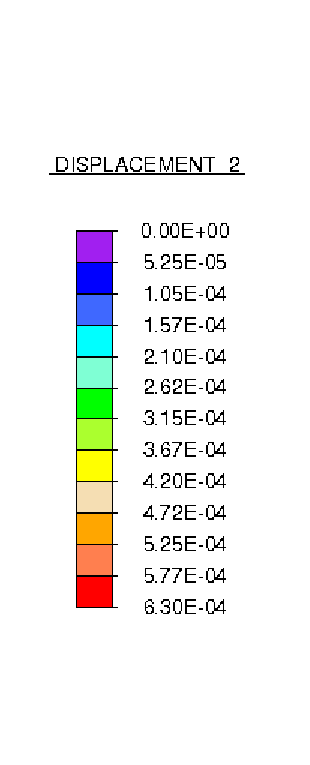
\includegraphics[width=0.15\textwidth]{dam2dc2}
\end{center}
\end{frame}
%%%%%%%%%%%%%%%%%%%%%%%%%%%%%%%%%%%%%%%%%%%%%%%%%%%%%%%%%%%%%%%%%%%%%%%%%%%%%%
\begin{frame}
\frametitle{Elasticidad 2D. Tensión plana}
\begin{itemize}
\item La condición de tensión plana es  $(\sigma_{zz}=0)$
\begin{align}
\left\{
\begin{array}{c}
\sigma_{xx} \\
\sigma_{yy} \\
\sigma_{xy}
\end{array}
\right\}&=
\left(
\begin{array}{ccc}
\frac{4\mu(\lambda+\mu)}{\lambda+2\mu} & \frac{2\lambda\mu}{\lambda+2\mu} & 0 \\
\frac{2\lambda\mu}{\lambda+2\mu} &\frac{4\mu(\lambda+\mu)}{\lambda+2\mu} &  0 \\
0           & 0       & \mu
\end{array}
\right)
\left\{
\begin{array}{c}
\varepsilon_{xx} \\
\varepsilon_{yy} \\
\varepsilon_{xy}
\end{array}
\right\} \\
\varepsilon_{zz}&=-\frac{\nu}{E} (\sigma_{xx}+\sigma_{yy})
\end{align}
\end{itemize}
\end{frame}
%%%%%%%%%%%%%%%%%%%%%%%%%%%%%%%%%%%%%%%%%%%%%%%%%%%%%%%%%%%%%%%%%%%%%%%%%%%%%%
\begin{frame}
\frametitle{Elasticidad 2D. Tensión plana}
\begin{center}
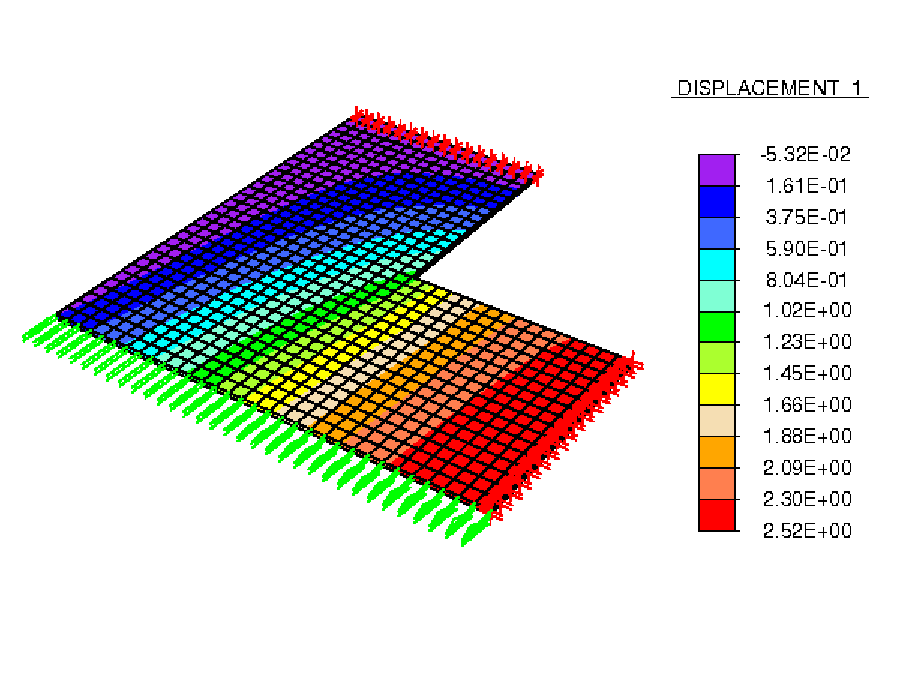
\includegraphics[width=0.50\textwidth]{L3D}
\hfill
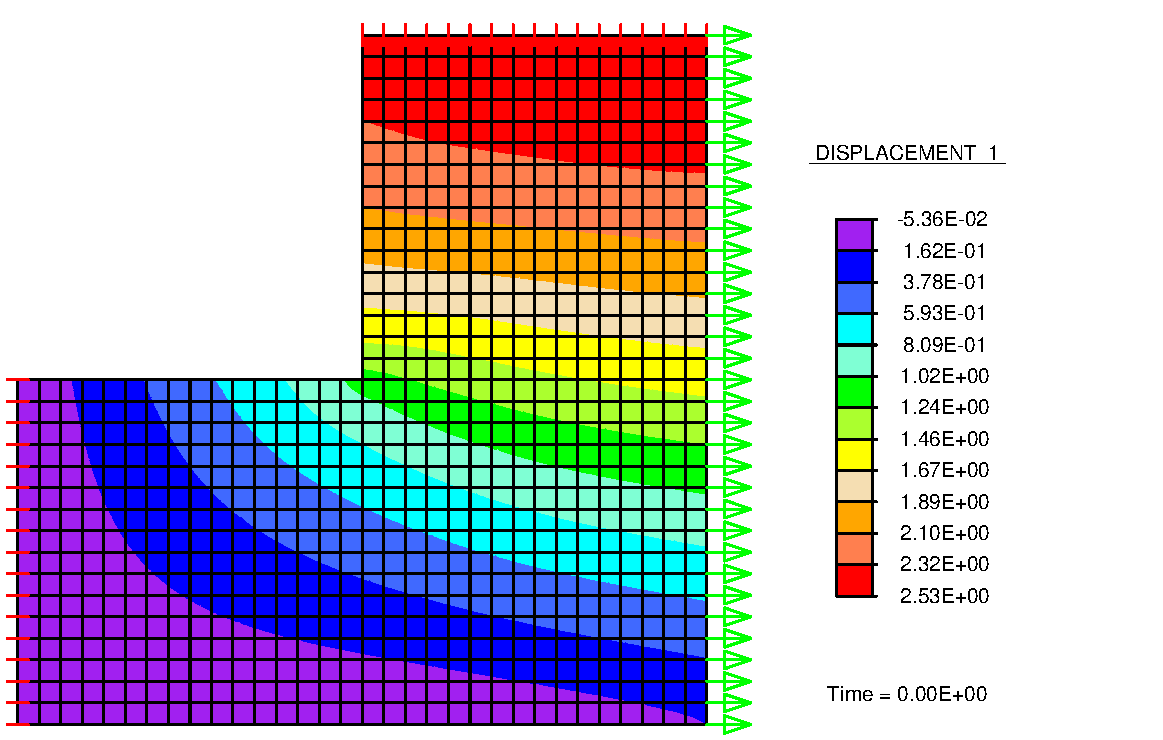
\includegraphics[width=0.45\textwidth]{L2D}
\end{center}
\end{frame}
%%%%%%%%%%%%%%%%%%%%%%%%%%%%%%%%%%%%%%%%%%%%%%%%%%%%%%%%%%%%%%%%%%%%%%%%%%%%%%
\begin{frame}
\frametitle{Elasticidad 2D. Problemas axilsimétricos}
\begin{itemize}
\item Se expresa en términos de las coordenadas cilíndricas $r$ (radial),
$z$ (axial) y $\theta$ (circunferencial).

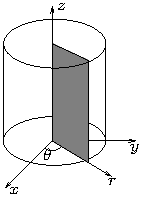
\includegraphics{axisim1}

\item Condición de simetría axial: todas las variables son independientes de 
$\theta$ y
además: $u_{\theta}$=0, $\varepsilon_{r \theta}=\varepsilon_{z \theta}=0$
\item En todos los integrandos hay que considerar un factor de $2 \pi r$
\end{itemize}
\end{frame}
%%%%%%%%%%%%%%%%%%%%%%%%%%%%%%%%%%%%%%%%%%%%%%%%%%%%%%%%%%%%%%%%%%%%%%%%%%%%%%
\begin{frame}
\frametitle{Elasticidad 2D. Problemas axilsimétricos}
\begin{itemize}
\item Relación tensión - deformación
\begin{equation}
\left\{
\begin{array}{c}
\sigma_{rr} \\
\sigma_{zz} \\
\sigma_{rz} \\
\sigma_{\theta \theta}
\end{array}
\right\}=
\left(
\begin{array}{cccc}
\lambda+2\mu & \lambda     & 0 & \lambda \\
\lambda     & \lambda+2\mu & 0 & \lambda \\
0           & 0       & \mu& 0 \\
\lambda     & \lambda & 0 & \lambda+2\mu
\end{array}
\right)
\left\{
\begin{array}{c}
\varepsilon_{rr} \\
\varepsilon_{zz} \\
\varepsilon_{rz} \\
\varepsilon_{\theta \theta}
\end{array}
\right\}
\end{equation}
\item La matriz $\mathbf{B}$ ( de interpolación del campo de deformaciones)
es:
\begin{equation}
\mathbf{B}=
\left(
\begin{array}{cc}
N_{a,r} & 0       \\
0       & N_{a,z} \\
N_{a,z} & N_{a,r} \\
\frac{N_a}{r}&0
\end{array}
\right) \qquad a=1 \ldots n_{\textrm{nen}}
\end{equation}
\end{itemize}
\end{frame}
%%%%%%%%%%%%%%%%%%%%%%%%%%%%%%%%%%%%%%%%%%%%%%%%%%%%%%%%%%%%%%%%%%%%%%%%%%%%%%
\begin{frame}
\frametitle{Elasticidad 2D. Problemas axilsimétricos}
\begin{center}
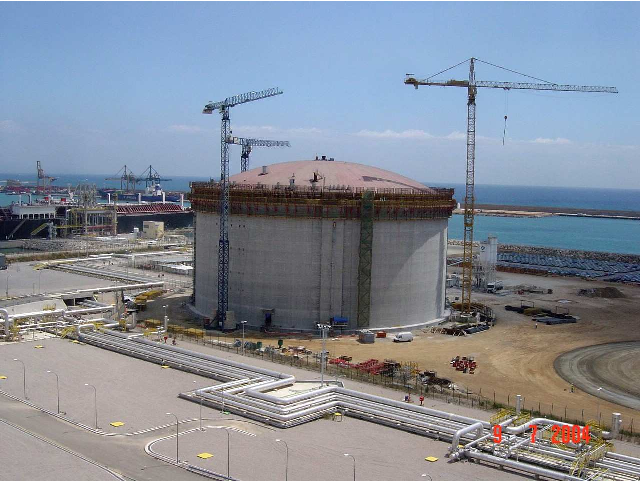
\includegraphics[width=0.8\textwidth]{tn_lng_tank2}
\end{center}
\end{frame}
%%%%%%%%%%%%%%%%%%%%%%%%%%%%%%%%%%%%%%%%%%%%%%%%%%%%%%%%%%%%%%%%%%%%%%%%%%%%%%
\begin{frame}
\frametitle{Elasticidad 3D}
\begin{itemize}
\item Relación tensión -  deformación
\begin{small}
\begin{equation}
\left\{
\begin{array}{c}
\sigma_{xx} \\
\sigma_{yy} \\
\sigma_{zz} \\
\sigma_{yz} \\
\sigma_{xz} \\
\sigma_{xy}
\end{array}
\right\}=
\left(
\begin{array}{cccccc}
\lambda + 2 \mu & \lambda       & \lambda       & 0     & 0     & 0     \\
\lambda         & \lambda+2 \mu & \lambda       & 0     & 0     & 0     \\
\lambda         & \lambda       & \lambda+2 \mu & 0     & 0     & 0     \\
0               & 0             & 0             & \mu   & 0     & 0     \\
0               & 0             & 0             & 0     & \mu   & 0     \\
0               & 0             & 0             & 0     & 0     & \mu   
\end{array}
\right)
\left\{
\begin{array}{c}
\varepsilon{xx} \\
\varepsilon{yy} \\
\varepsilon{zz} \\
\varepsilon{yz} \\
\varepsilon{xz} \\
\varepsilon{xy}
\end{array}
\right\}
\end{equation}
\end{small}
\end{itemize}
\end{frame}
%%%%%%%%%%%%%%%%%%%%%%%%%%%%%%%%%%%%%%%%%%%%%%%%%%%%%%%%%%%%%%%%%%%%%%%%%%%%%%
\begin{frame}
\frametitle{Elasticidad 3D}
\begin{center}
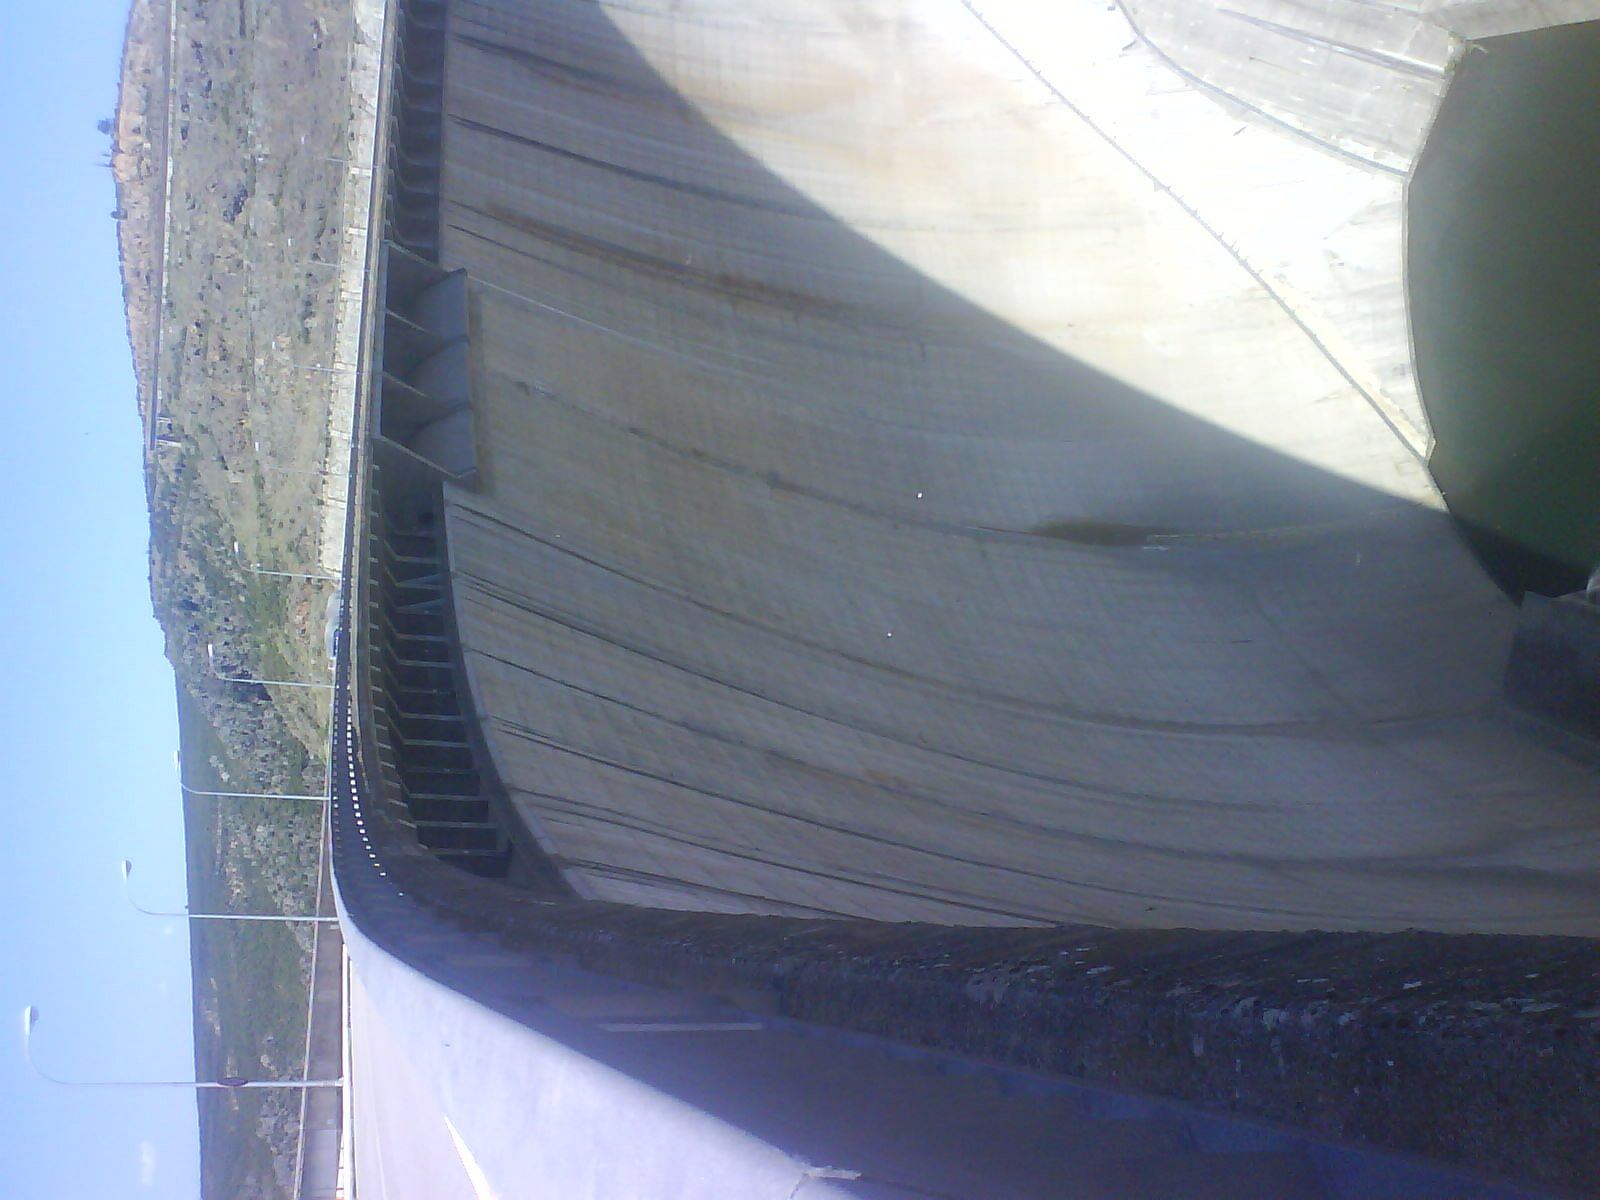
\includegraphics[width=0.85\textheight,angle=-90]{el_atazar_02}
\end{center}
\end{frame}
%%%%%%%%%%%%%%%%%%%%%%%%%%%%%%%%%%%%%%%%%%%%%%%%%%%%%%%%%%%%%%%%%%%%%%%%%%%%%%
\end{document}
